\section*{Math 202A - HW9 - Dan Davison - \texttt{ddavison@berkeley.edu}}

\begin{mdframed}
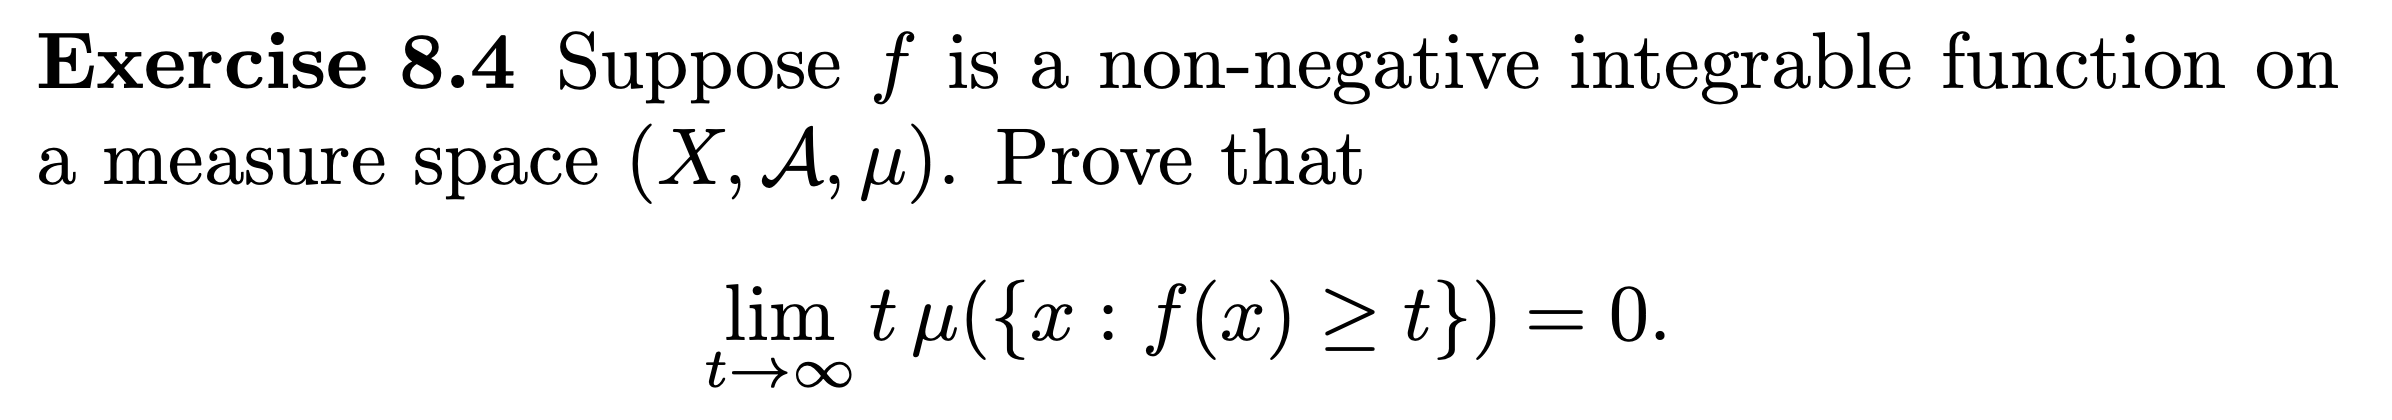
\includegraphics[width=400pt]{img/analysis--berkeley-202a-hw09-210c.png}
\end{mdframed}

\begin{proof}
  Let $t_1, t_2, \ldots \in \R$ with $\limn t_n = \infty$ and define $A_n = \{x ~:~ f(x) > t_n\}$.

  Thus we have $\lim_{t\to\infty} t ~ \mu\big(\{x ~:~ f(x) \geq t\}\big) = \limn t_n \mu(A_n)$, since the limit
  is the same along any sequence.

  Note that $f\ind_{A_n} \to 0$, since $A_n \downarrow \emptyset$, and note also that $f\ind_{A_n} \leq f$ for
  all $n$.

  Therefore
  \begin{align*}
    \limn t_n \mu(A_n)
    &\leq \limn \int f\ind_{A_n} \\
    &= \int \limn f\ind_{A_n}             &\text{by the dominated convergence theorem}\\
    &= \int \limn 0 \\
    &= 0.
  \end{align*}
\end{proof}

\newpage
\begin{mdframed}
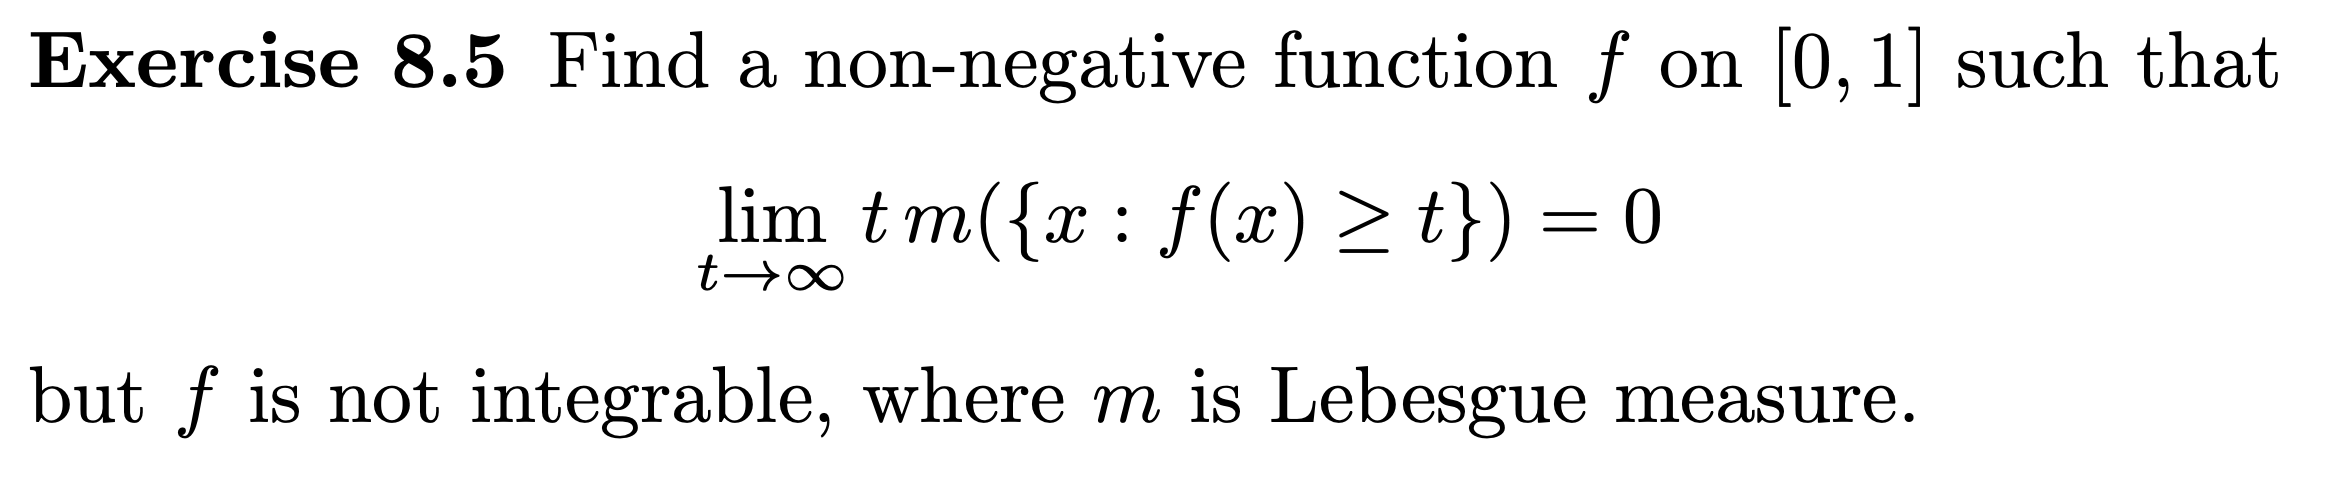
\includegraphics[width=400pt]{img/analysis--berkeley-202a-hw09-b0e8.png}
\end{mdframed}

\begin{proof}

\end{proof}
\newpage

\begin{mdframed}
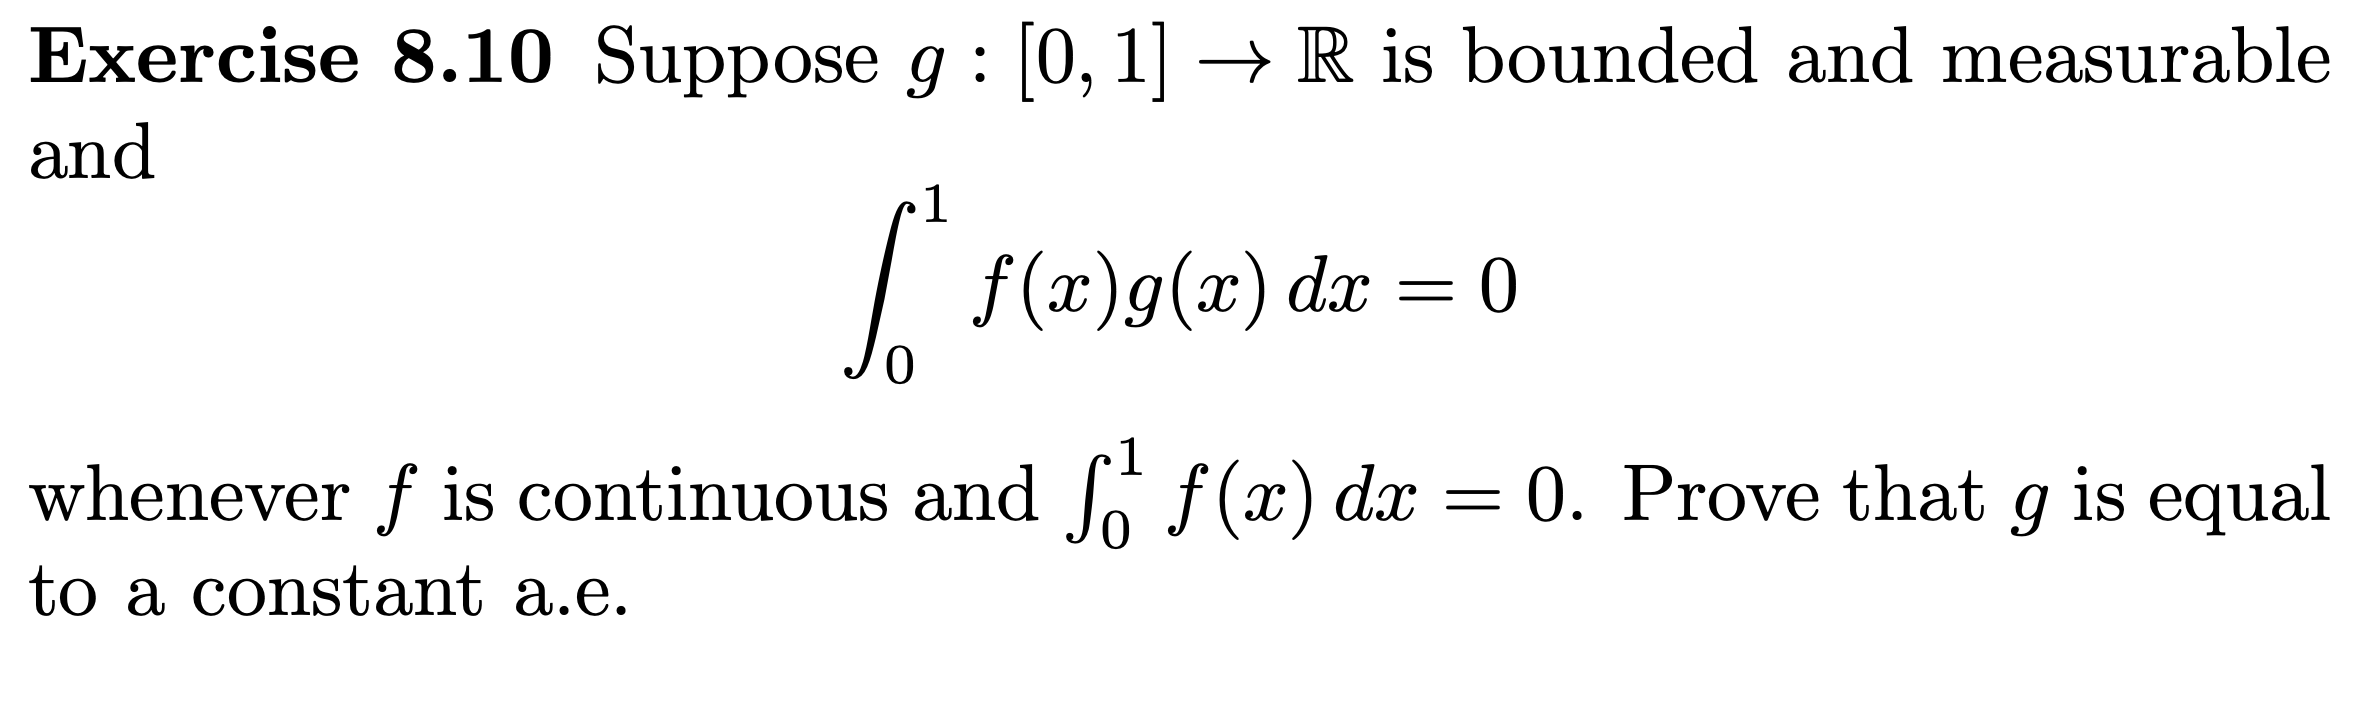
\includegraphics[width=400pt]{img/analysis--berkeley-202a-hw09-113a.png}
\end{mdframed}

\begin{proof}
  Let $g: [0, 1] \to \R$ be a function that is not constant a.e.

  We will construct an $f$ such that $\int_0^1 f = 0$ and $\int_0^1 fg \neq 0$, thus proving the result by
  contradiction.

  Let $f(x) = x - 1/2$. Note that $\int_0^1 f = 0$.

  If $\int_0^1 fg \neq 0$ then we are done.

  Alternatively, we have $\int_0^1 fg = 0$, or equivalently
  \begin{align*}
    \int_0^{1/2} fg + \int_{1/2}^1 fg = 0.
  \end{align*}


  and let $g^*$ be a continuous approximation to $g$.



  If $\int g^* = 0$ then we are done since $\int_0^1 fg = \int_0^1 (g^*)^2 > 0$.


\end{proof}


\begin{proof}
  We have that for every continuous function $f$ with $\int_0^1 f = 0$ then $\int_0^1 fg = 0$.

  It follows that for every continuous function $f$ with $\int_0^1 f = 0$ and for all $a, b \in \R$
  \begin{align*}
    \int_0^1 af + bfg = 0.
  \end{align*}
  It is given that $g$ is bounded, and we see that $f$ is bounded also since it is continuous on a compact set.

  Let $L, M$ be such that $L \geq |g|$ and $M \geq |f|$. Then we have that


\end{proof}


\begin{proof}
  Let $f_1 \neq f_2$ be continuous with $\int_0^1 f_1 = \int_0^1 f_2 = 0$.

  We have that
  \begin{align*}
    \int_0^1 f_1g = \int_0^1 f_2g = 0.
  \end{align*}

  For example, let $f_n(x) = n(x - 1/2)$. Then
  \begin{align*}
    \int_0^1 f_n(x) \dx = n\int_0^1 x \dx - \frac{n}{2} = \frac{n}{2} - \frac{n}{2} = 0.
  \end{align*}
  Let
  \begin{align*}
    g(x) =
    \begin{cases}
      -c & x \leq 1/2 \\
      +c  & x > 1/2.
  \end{cases}
  \end{align*}
  Then
  \begin{align*}
    \int_0^1 f_n(x) g(x)
    = -cn\int_0^{1/2}(x - 1/2) \dx + cn\int_{1/2}^1(x - 1/2) \dx
    = 0.
  \end{align*}
\end{proof}








\begin{remark}
  As a sanity check note that the required behavior with continuous $f$ does obtain
  \begin{enumerate}
  \item if $g$ is equal to a constant a.e.: if $c \in \R$ and $g = c$ a.e. then $\int_0^1 f g = c \int_0^1 f = 0$,
  \item if $f = 0$.
  \end{enumerate}
\end{remark}


\begin{proof}
  Suppose $g: [0, 1] \to [0, \infty]$ is bounded and measurable.

  Let $\lambda(E) = \int_E g(x) \dx$ for a Borel set $E \subseteq [0, 1]$.

  Then by HW7 Ex. 1 we have that $\lambda$ is a measure on $[0, 1]$ and
  \begin{align*}
    \int_0^1 f(x)g(x) \dx = \int_0^1 f \d\lambda.
  \end{align*}
  Thus the question is equivalent to positing the existence of a measure $\lambda$ such that for every
  continuous function $f$ with $\int_0^1 f(x) \dx = 0$ we have
  \begin{align*}
    \int_0^1 f \d\lambda = 0.
  \end{align*}

\end{proof}




\begin{proof}
  Let $\ms F = \{f: [0, 1] \to \R ~:~ f \text{~is continuous}, \int_0^1 f(x) \dx = 0 \}$.

  Is $\ms F$ (in an appropriate sense) full rank, such that if a function $g$ is orthogonal to every element
  of $f$ then $g$ must be the zero function? (And then some argument allowing $g$ to be any constant a.e.
  function).
\end{proof}


Suppose condition A(f, g) is true whenever f satisfies condition B. Prove that g satisfies condition C.

Claim: If (f satisfies condition B) => A(f, g), then g satisfies condition C.

Proof:

We must show

(1) if not B(f) then C(g)

(2) if B(f) and


\begin{claim*}
  Suppose $g: [0, 1] \to \R$ is bounded and measurable.

  Suppose further that, if $f$ is continuous and $\int_0^1 f = 0$, then
  \begin{align*}
    \int_0^1 f g = 0.
  \end{align*}

  Prove that $g$ is equal to a constant a.e.
\end{claim*}

\begin{intuition}
  We have an unknown function $g: [0, 1] \to \R$.

  We are told that whenever $g$ is integrated against a continuous function $f$ for which $\int_0^1 f = 0$, the
  result is zero.

  We must prove that $g$ is equal to a constant a.e.


\end{intuition}

\begin{proof}
  Suppose $g$ is not equal to a constant a.e.

\end{proof}


\newpage
\begin{mdframed}
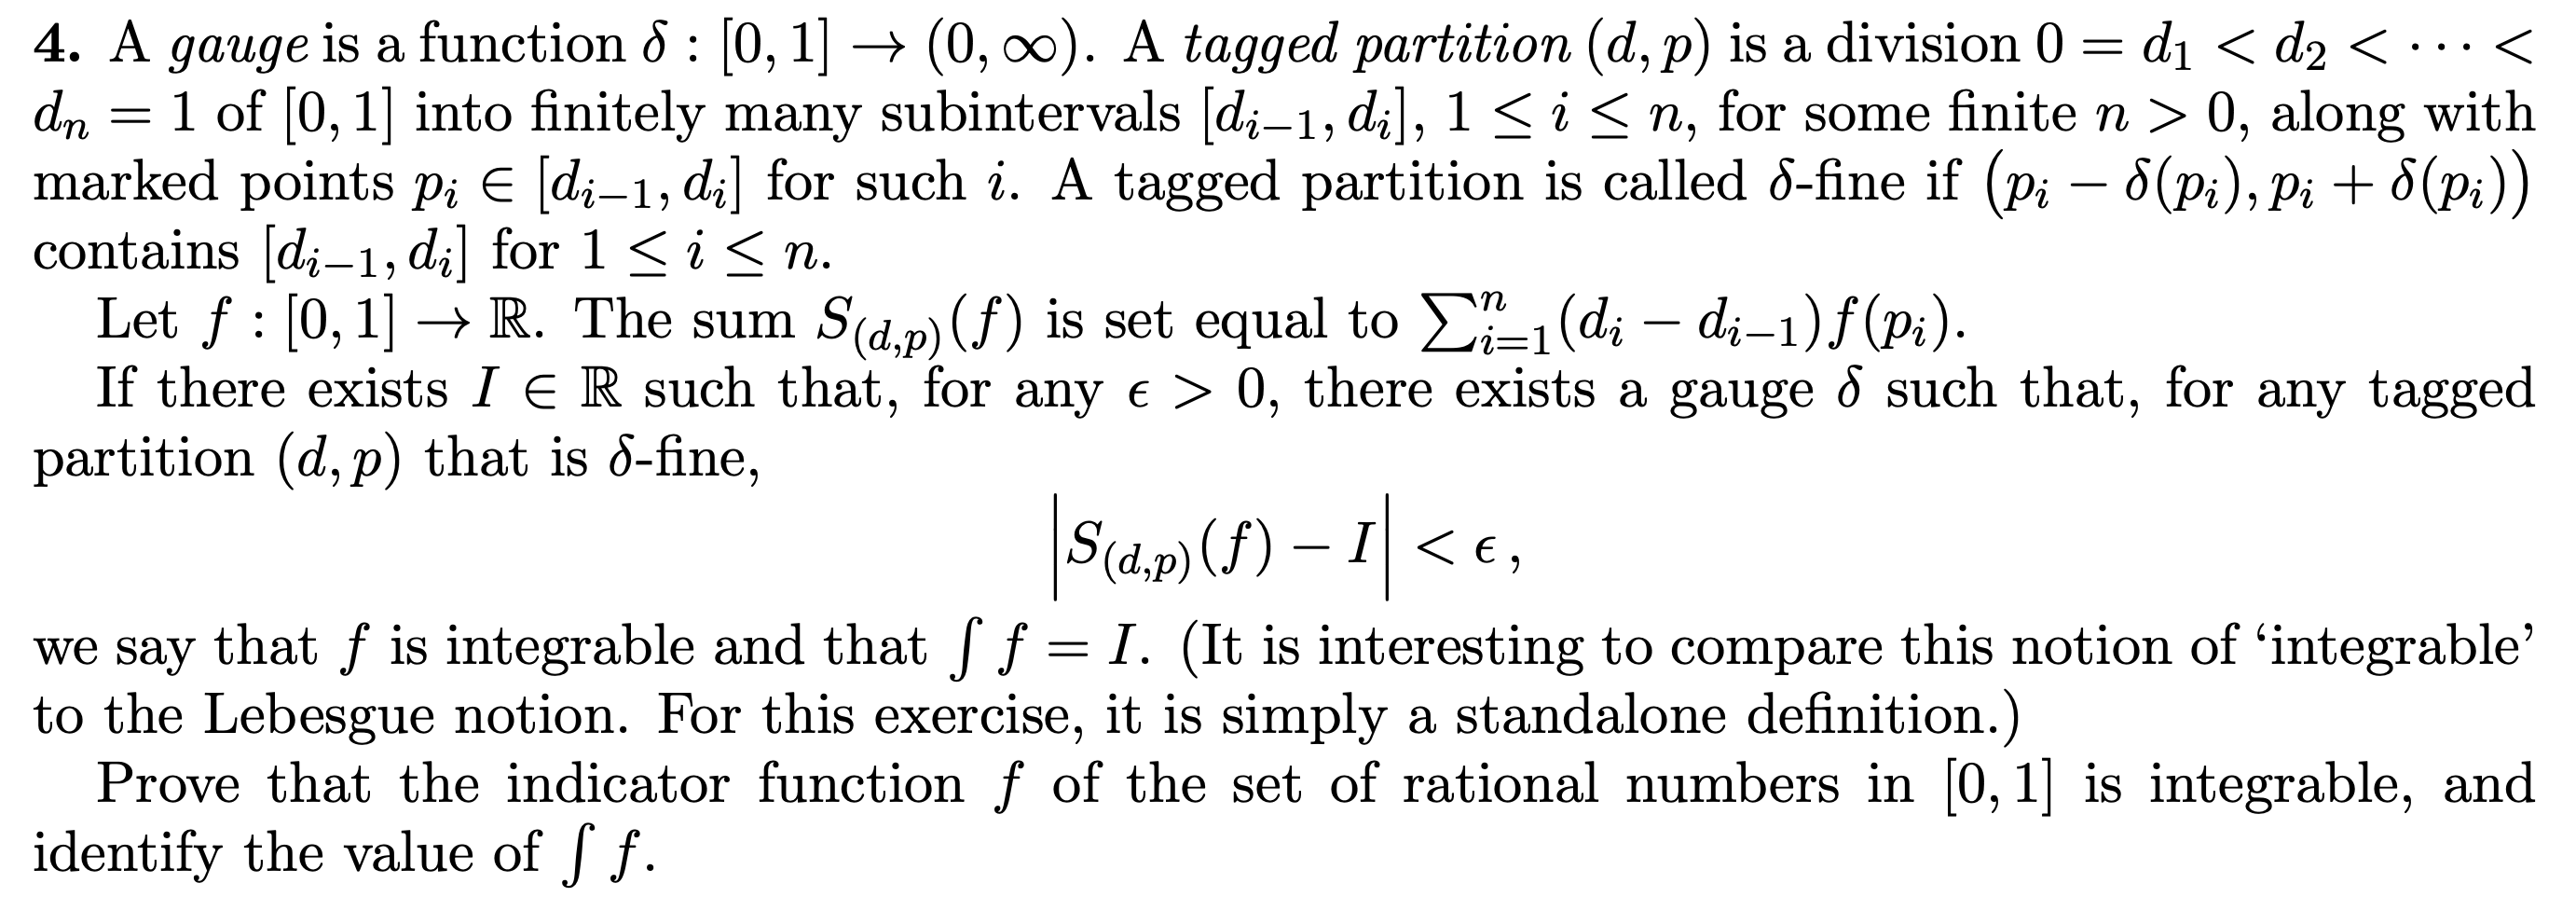
\includegraphics[width=400pt]{img/analysis--berkeley-202a-hw09-955c.png}
\end{mdframed}

\begin{claim*}
  Henstock-Kurzweil $\int \ind_\Q \neq 0$
\end{claim*}

\begin{proof}
  We claim that $\int \ind_\Q = 0$.

  Let $\eps > 0$.

  We must prove that there exists a gauge $\delta$ such that for all tagged partitions $(d, p)$ if $(d, p)$
  is $\delta$-fine then
  \begin{align*}
    \sum_{i=1}^n (d_i - d_{i-1})\ind_\Q(p_i) < \eps.
  \end{align*}



  Equivalently we must prove that there exists a gauge $\delta$ such that
  \begin{align*}
    \max_{(d, p) \delta\text{-fine}} \Bigg( \sum_{\{i ~:~ i \in \{1, \ldots, n\}, p_i \in \Q\}} (d_i - d_{i-1}) \Bigg) < \eps,
  \end{align*}

  where we were able to remove the absolute value operator because the $d_i$ are increasing.

  Note that the tagged partition that maximises this quantity will be one for which $p_i \in \Q$ for
  all $i \in \{1, \ldots, n\}$.

  Therefore we must prove that there exists a gauge $\delta$ such that
  \begin{align*}
    \max_{(d, p) \delta\text{-fine}, ~\forall i ~ p_i \in \Q} \sum_{i=1}^n (d_i - d_{i-1}) < \eps,
  \end{align*}



  Note that if $(d, p)$ is a tagged partition such that $p_i \notin \Q$ for all $i \in \{1, \ldots, n\}$, then
  the condition is true. Therefore we need only consider tagged partitions for which some $p_i$ are rational.

  Let $\delta = c/2$ be a constant function.

  Then a tagged partition $(d, p)$ is $\delta$-fine if $d_{i} - d_{i-1} < c$ for all $i$.

  Let   $(d, p)$ be such that $d_{i} - d_{i-1} < c$ for all $i$.

\end{proof}










\begin{proof}
  \begin{align*}
    \hline
    &\forall \eps > 0 ~~ \exists \delta ~~ \forall (d, p) ~~ \delta\text{-fine}(d, p) ~~ \Big|\sum_{\{i ~:~ i \in \{1, \ldots, n\}, p_i \in \Q\}} (d_i - d_{i-1})\Big| < \eps
  \end{align*}

\begin{align*}
  &\eps > 0 \\
  \hline
  &\exists \delta ~~ \forall (d, p) ~~ \delta\text{-fine}(d, p) ~~ \Big|\sum_{\{i ~:~ i \in \{1, \ldots, n\}, p_i \in \Q\}} (d_i - d_{i-1})\Big| < \eps
  \end{align*}
\end{proof}
\newpage
\begin{mdframed}
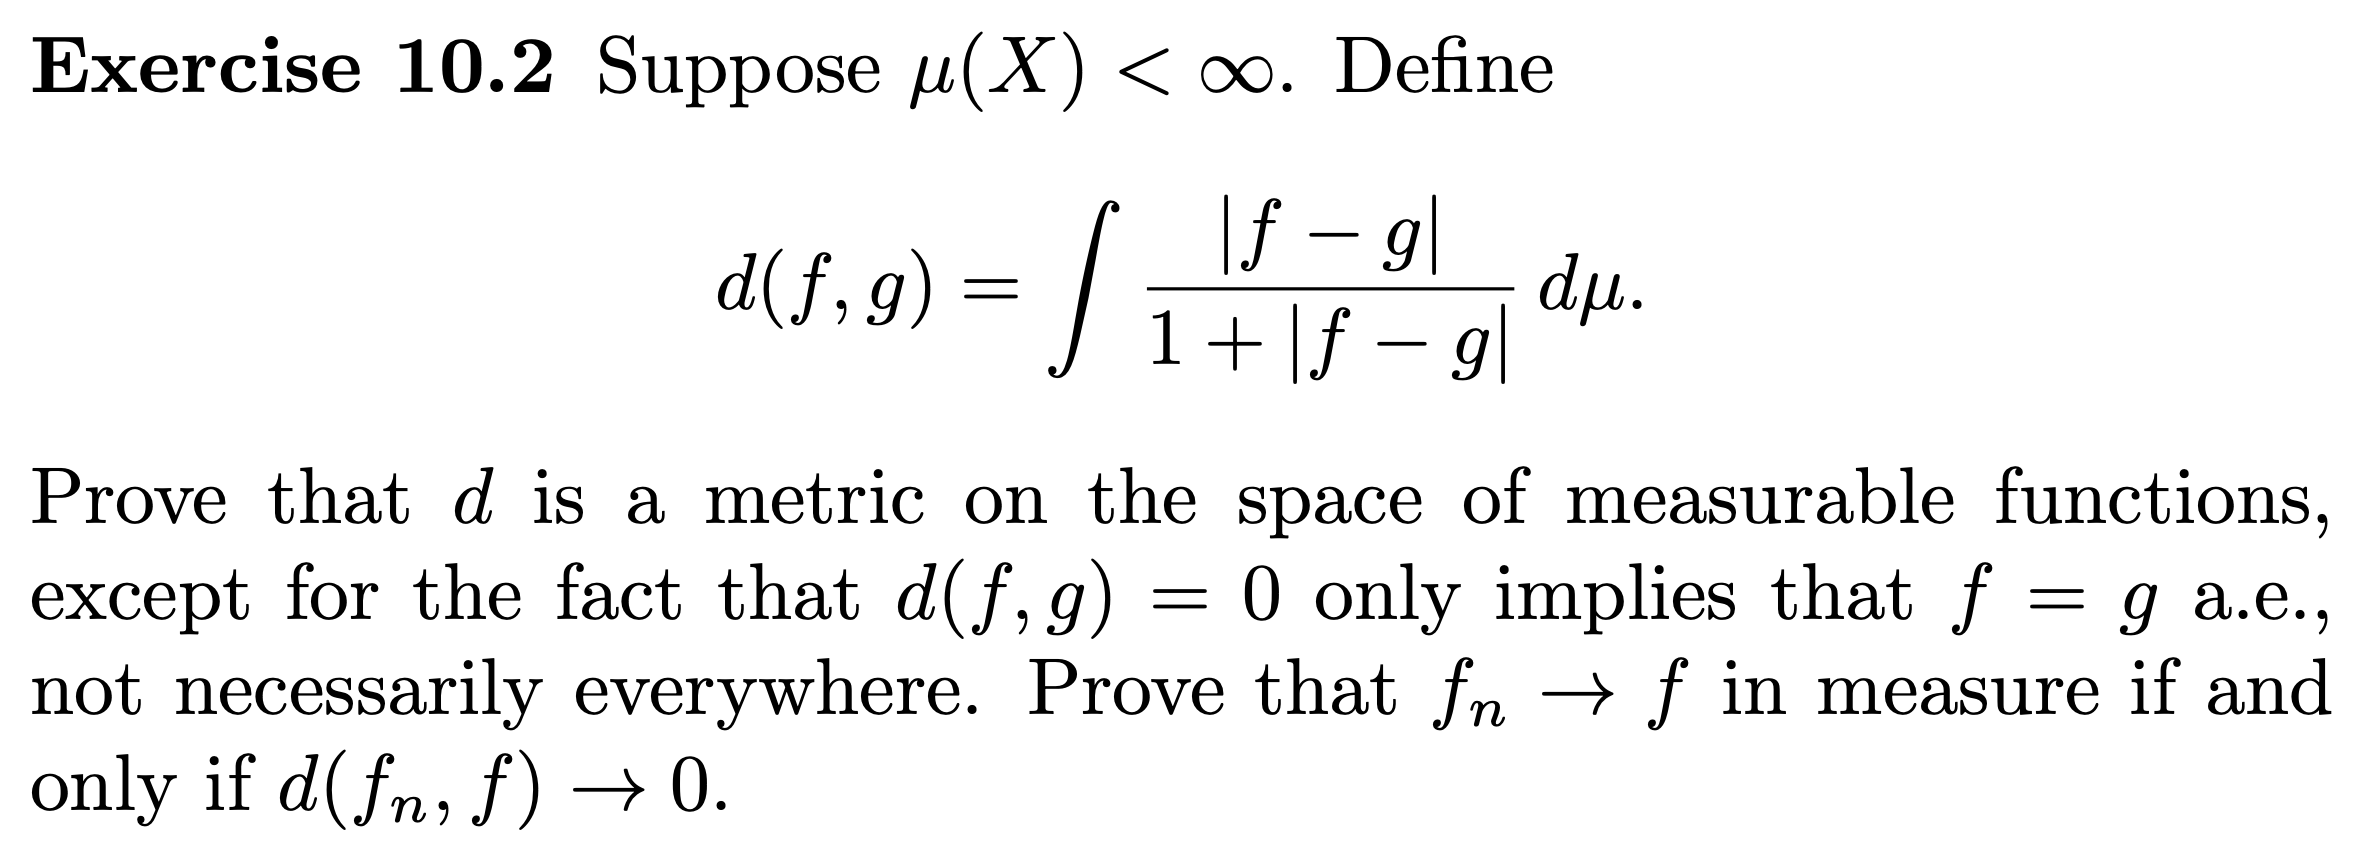
\includegraphics[width=400pt]{img/analysis--berkeley-202a-hw09-b4e1.png}
\end{mdframed}

\begin{claim*}
  $d$ is a metric on the space of measurable functions except for the fact that $d(f, g) = 0$ implies $f = g$
  a.e., not necessarily everywhere.
\end{claim*}

\begin{proof}~\\
  \begin{enumerate}
  \item {\bf identity of indiscernibles}\\
    Note that $\frac{|f - g|}{1 + |f - g|} \geq 0$. Therefore
    if $d(f, g) = \int\frac{|f - g|}{1 + |f - g|} = 0$ then $|f - g| = 0$ a.e., and therefore $f = g$ a.e.

    Conversely, if $f = g$ a.e. then $|f - g| = 0$ a.e. and we have $d(f, g) = 0$.

  \item {\bf symmetry}\\
    $d(f, g) = \int \frac{|f - g|}{1 + |f - g|} = \int \frac{|g - f|}{1 + |g - f|} = d(g, f)$

  \item {\bf triangle inequality}
    \begin{align*}
      d(f, h)
      &= \int \frac{|f - h|}{1 + |f - h|} \\
      &= \int \frac{|f - g + g - h|}{1 + |f - g + g - h|} \\
      &\leq \int \frac{|f - g| + |g - h|}{1 + |f - g| + |g - h|} \\
      &< \int \frac{|f - g|}{1 + |f - g|} + \int \frac{|g - h|}{1 + |g - h|} \\
      &= d(f, g) + d(g, h)
    \end{align*}
  \end{enumerate}
\end{proof}

\begin{lemma}\label{10-2-lemma}
  $d(f_n, f) \to 0$ if and only if $f_n \to f$ a.e.
\end{lemma}

\begin{proof}
  Since $0 \leq \frac{|f_n - f|}{1 + |f_n - f|} \leq 1$ we may appply the dominated convergence theorem,
  yielding
  \begin{align}
    \limn d(f_n, f)
    &= \limn \int \frac{|f_n - f|}{1 + |f_n - f|} \nonumber\\
    &= \int \limn \frac{|f_n - f|}{1 + |f_n - f|} \nonumber\\
    &= \int \frac{\limn |f_n - f|}{1 + \limn |f_n - f|}. \label{10-2-eqn}
  \end{align}
  First suppose that $d(f_n, f) \to 0$. Then, since for all $n$ the integrand on the RHS of \eqref{10-2-eqn} is
  non-negative, and the denominator of the integrand on the RHS of \eqref{10-2-eqn} is strictly positive, we
  have $\limn |f_n - f| = 0$ a.e. or in other words $f_n \to f$ a.e.

  Converself, suppose that $f_n \to f$ a.e. Then the integrand on the RHS of \eqref{10-2-eqn} is zero and we
  have $d(f_n, f) \to 0$.
\end{proof}


\begin{claim*}
 If $d(f_n, f) \to 0$ then $f_n \to f$ in measure.
\end{claim*}

\begin{proof}
  From lemma \ref{10-2-lemma} we have $f_n \to f$ a.e. Therefore $f_n \to f$ in measure.
\end{proof}

\begin{claim*}
  If $f_n \to f$ in measure then $d(f_n, f) \to 0$.
\end{claim*}

\begin{proof}
  Suppose that $f_n \to f$ in measure.

  Let $\eps > 0$ and define $A_{\eps, n} = \{x ~:~ |f_n(x) - f| > \eps\}$.

  Since $0 \leq \ind_{A_{\eps, n}} \leq 1$ and $\int 1 = \mu(X) < \infty$ we may apply the dominated
  convergence theorem, yielding
  \begin{align*}
    0 = \limn \mu(A_{\eps, n}) = \limn \int \ind_{A_{\eps, n}} = \int \limn \ind_{A_{\eps, n}}.
  \end{align*}
  Since the integrand $\limn \ind_{A_{\eps, n}}$ is non-negative we have
  \begin{align*}
    \limn \ind_{A_{\eps, n}}(x) = 0 \ae,
  \end{align*}
  or equivalently
  \begin{align*}
    \limn |f_n(x) - f(x)| \leq \eps \ae
  \end{align*}
  Thus since $\eps$ was arbitrary we have
  \begin{align*}
    \limn |f_n(x) - f(x)| = 0 \ae
  \end{align*}
  and therefore
  $f_n \to f$ a.e.

  The claim then follows from lemma \ref{10-2-lemma}.
\end{proof}


\newpage
\begin{mdframed}
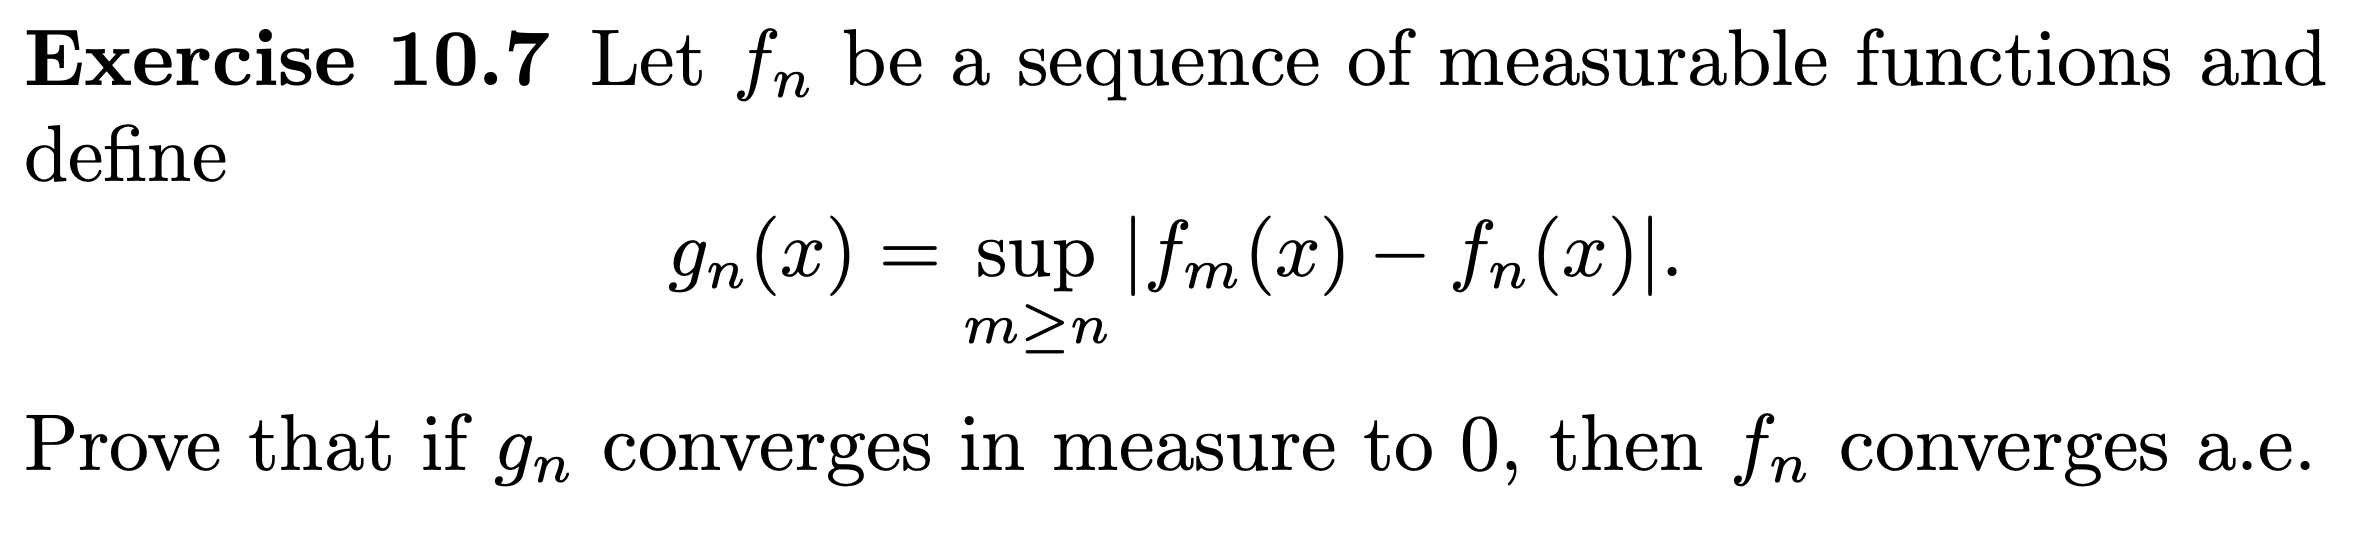
\includegraphics[width=400pt]{img/analysis--berkeley-202a-hw09-ea17.png}
\end{mdframed}